\documentclass{report}
\usepackage[letterpaper,portrait,margin=2cm]{geometry}
\usepackage{titlesec}
\usepackage{amsmath,amssymb,amsthm}
\usepackage{tabularx}
\usepackage{enumitem}
\usepackage{indentfirst}
\usepackage{dsfont}
\usepackage{tikz}
\usepackage{hyperref}
\usepackage{mathtools}
\usepackage{mathrsfs}
\usepackage{enumitem}
\usepackage{wasysym}

\hypersetup{
	colorlinks=false
}

\renewcommand{\contentsname}{Table des mati\`eres}

\title{MAT141 - \'El\'ements d'alg\`ebre

Donn\'e par Jean-Philippe Burelle}
\author{Julien Houle}
\date{Automne 2025}

\newcounter{cours}
\setcounter{cours}{1}
\newcommand*{\cours}{\section*{Cours \thecours}\stepcounter{cours}}

\newcommand*{\abs}[1]{\left| #1 \right|}
\newcommand*{\card}[1]{\left| #1 \right|}

\renewcommand{\thesection}{Section \arabic{chapter}.\arabic{section}}
\renewcommand{\thesubsection}{}
\renewcommand{\thesubsubsection}{}

\titleformat{\chapter}[hang]{\bfseries\huge\centering}{Chapitre \arabic{chapter}}{1em}{}[]
\titleformat{\section}[hang]{\bfseries\large}{}{1em}{}[]
\titleformat{\subsection}[hang]{\bfseries\normalsize}{}{0pt}{}[]
\titleformat{\subsubsection}[hang]{\slshape\normalsize}{}{0pt}{}[]

\newtheorem*{thm}{Th\'eor\`eme}
\newtheorem*{lem}{Lemme}
\newtheorem*{prop}{Proposition}
\theoremstyle{definition}
\newtheorem*{defin}{D\'efinition}
\theoremstyle{remark}
\newtheorem*{exem}{Exemple}
\newtheorem*{exer}{Exercice}
\newtheorem*{nota}{Notation}
\newtheorem*{rema}{Remarque}
\newtheorem*{rappel}{Rappel}

\begin{document}
	\maketitle
	\tableofcontents
	\newpage

	\chapter{Ensembles}
	\cours
	Id\'ee: ensemble=patate

	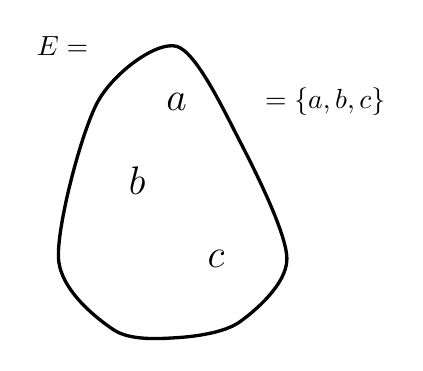
\begin{tikzpicture}
		\path[smooth cycle,very thick,draw=black] plot coordinates {(0,-.3) (-1,-1) (-1.5,-3) (-.8,-3.9) (0,-4) (.8,-3.8) (1.4,-3) (.8,-1.5)};
		\node[font=\Large] () at (0,-1) {$a$};
		\node[font=\Large] () at (-.5,-2) {$b$};
		\node[font=\Large] () at (.5,-3) {$c$};
		\node[anchor=east] () at (-1,-.3) {$E=$};
		\node[anchor=west] () at (1,-1) {$=\{a,b,c\}$};
	\end{tikzpicture}

	\begin{nota}
		$E \subseteq F \Leftarrow \forall x \in E, x \in F$.
		\begin{rema}
			$E \subseteq E$.
		\end{rema}
	\end{nota}

	\begin{nota}
		La cardinalit\'e d'un ensemble, $\card{E}$, est le nombre d'\'el\'ements d'un ensemble.
	\end{nota}

	\begin{defin}
		D\'efinition d'un ensemble par \emph{compr\'ehension}: $E=\left\lbrace n \in \mathbb{Z} \middle| 1 \leq n \leq 20 \right\rbrace$.
	\end{defin}

	\begin{nota}
		$E=F \Leftrightarrow E \subseteq F$ et $F \subseteq E$.
	\end{nota}

	\begin{defin}
		Produit cart\'esien: $E \times F=\left\lbrace (x,y) \middle| x \in E, y \in F \right\rbrace$.
	\end{defin}

	\begin{defin}
		Fonction/Application

		$f: A \to B$, $A$ et $B$ des ensembles, associe \`a \emph{chaque} $x \in A$ un \emph{unique} \'el\'ement $f(x) \in B$.
	\end{defin}

	\cours
	\begin{rappel}
		~

		\begin{tabularx}{.9\textwidth}{cl>{\raggedright\arraybackslash}X}
			\textbullet&Ensemble&collection d'objets\\
			\textbullet&$\in$&``\'el\'ement'' d'un ensemble\\
			\textbullet&\emph{sous-ensemble} $(\subseteq)$&$E \subseteq F$ si $x \in E$ \emph{implique} $x \in F$\\
			\textbullet&$E=F$&ssi $E \subseteq F$ et $F \subseteq E$\\
			\textbullet&$\cup$&union\\
			&$\cap$&intersection\\
			\textbullet&$E \times F$&produit cart\'esien (paires $(x,y)$)\\
			\textbullet&$f:E \to F$&\emph{fonction} ou \emph{application}, associe \`a \underline{chaque $x \in E$} un unique $\underline{f(x)} \in F$, image de $x$ par $f$\\
			\textbullet&$\mathds{1}$&$\mathds{1}_E:E \to E$ est d\'efinie comme $\mathds{1}_E(x)=x$
		\end{tabularx}
	\end{rappel}


	\subsection{Mani\`eres de d\'efinir une fonction}
	\begin{itemize}[noitemsep]
		\item \'enum\'erer $f(x)$ pour chaque $x \in E$
		\item donner une formule

		une formule ne d\'efinit pas tjrs une fonction, elle doit \^etre valide pour chaque $x$ de l'ensemble de d\'epart.
		\item en mots (d\'ecrire la valeur pour chaque $x \in E$)
		\item m\'elange de formule et mots
	\end{itemize}

	\begin{defin}
		Une fonction $f:E \to F$ est \emph{inversible} s'il existe une fonction $\underbrace{g:F \to E}_{*}$ telle que $\underbrace{g(f(x))=x}_{**}$ pour tout $x \in E$ et $\underbrace{f(g(y))=y}_{***}$ pour tout $y \in F$.
	\end{defin}

	\begin{exem}
		$f:\mathbb{Z} \to \mathbb{Z}$, $f(x)=x+1$ est inversible d'inverse $g(y)=y-1$

		\begin{proof}[d\'emo.]
			~

			On v\'erifie que
			\begin{align*}
				g(f(x))&= x& g(f(x))&= g(x+1)\\
				&&&= (x+1)-1\\
				&&&= x\\
				f(g(y))&= y& f(g(y))&= f(y-1)\\
				&&&= (y-1)+1\\
				&&&= y
			\end{align*}
		\end{proof}
	\end{exem}

	\begin{prop}
		Si $f$ admet un inverse, celui-ci est unique.

		\begin{proof}[d\'emo.]
			~

			Supposons que $g_1$ et $g_2$ sont tous deux inverses de $f$ et montrons qu'elles sont \'gales.

			(Pour d\'emontrer que deux fonctions sont \'egales, il suffit de montrer que $g_1(y)=g_2(y)$ pour tout $y \in F$)

			Soit $y \in F$.

			On a
			\begin{align*}
				g_1(y)&\overbrace{=}^{***} g_1(\underbrace{f(g_2(y))}_{*})\\
				&\overbrace{=}^{**} g_2(y)
			\end{align*}
		\end{proof}
	\end{prop}

	\begin{defin}
		Si $f:E \to F$ et $g:F \to G$, alors la compos\'ee de $f$ et $g$ est la fonction $g \circ f:E \to G$ d\'efinie par la formule $g \circ f(x)=g(f(x))$.
	\end{defin}

	\begin{defin}[Red\'efinition de l'inverse]
		$g \circ f=\mathds{1}_E$

		$f \circ g=\mathds{1}_F$
	\end{defin}

	\begin{exem}
		$A=\{a,b,c\}$

		$B=\{d,e,f\}$

		$f:A \to B$, $a \mapsto d, b \mapsto e, c \mapsto f$

		$g:B \to A$, $d \mapsto a, e \mapsto b, f \mapsto c$

		$g \circ f:A \to A$, $g \circ f(x)=x$, $g \circ f=\mathds{1}_A$.

		De la \^m mani\`ere, $f \circ g=\mathds{1}_B$.

		~

		Ainsi, $g$ est l'inverse de $f$.
	\end{exem}

	\begin{nota}
		On note $g=f^{-1}$ l'inverse de $f$.
	\end{nota}


	\begin{rappel}
		Pour trouver l'inverse d'une fonction $f:\mathbb{R} \to \mathbb{R}$ donn\'ee par une formule $f(x)=y$, on isole $x$ en fonction de $y$.
	\end{rappel}


	\begin{exem}
		\begin{align*}
			f(x)&= 3x-8\\
			y&= 3x-8\\
			y+8&= 3x\\
			\dfrac{y+8}{3}&= x\\
			g(y)&= \dfrac{y+8}{3}
		\end{align*}

		Dans un devoir, on commence par la formule de l'inverse et on v\'erifie $g(f(x))=x$ et $f(g(y))=y$.
	\end{exem}

	\begin{defin}
		On dit que $f:E \to F$ est une fonction \emph{injective} si $f(x_1)=f(x_2)$ implique $x_1=x_2$.
	\end{defin}

	\begin{defin}
		On dit que $f:E \to F$ est une fonction \emph{surjective} si pour tout $y \in F,~\exists~x \in E$ t.q. $f(x)=y$.
	\end{defin}

	\begin{defin}
		On dit que $f:E \to F$ est une fonction \emph{bijective} si elle est injective \textbf{et} surjective.
	\end{defin}

	\begin{exem}
		$f:\mathbb{R} \to \mathbb{R}^{\geq0}$, $f(x)=\abs{x}$

		$f$ n'est pas injective, car $f(1)=\abs{1}=1$ et $f(-1)=\abs{-1}=1$, mais $1 \neq -1$.

		$f$ est surjective, car soit $y \in \mathbb{R}^{\geq0}$, alors pour $x=y$, on a $f(x)=f(y)=\abs{y}=y$.

		~

		\[
		\begin{array}{rrcl}
			f:&\mathbb{N}&\to&\mathbb{N}\\
			&x&\mapsto&x+1
		\end{array}
		\]

		$f$ est injective:

		Soient $x_1,x_2 \in \mathbb{N}$.

		On suppose $f(x_1)=f(x_2)$.

		\begin{align*}
			x_1+1&= x_2+1\\
			x_1&= x_2
		\end{align*}

		$f$ n'est pas surjective

		$y=0\in\mathbb{N}$ n'est pas \'egal \`a $f(x)$ pour $x\in\mathbb{N}$. Si il existait $x$ avec $f(x)=0$, $x+1=0$, $x=-1$, $x \not\in \mathbb{N}$.

		~

		$f:\mathbb{R}\to\mathbb{R}$, $x \mapsto 2x+3$.

		$f$ est injective:

		Soient $x_1,x_2 \in \mathbb{R}$.

		supposons $f(x_1)=f(x_2)$, $2x_1+3=2x_2+3$, $2x_1=2x_2$, $x_1=x_2$.

		$f$ est surjective:

		Soit $y \in \mathbb{R}$.

		On cherche $x$ t.q. $f(x)=y$.

		Posons $x=\dfrac{y-3}{2} \in \mathbb{R}$.

		Alors, $f(x) = f\left( \dfrac{y-3}{2} \right) = 2 \cdot  \dfrac{y-3}{2} + 3 = y-3+3 = y$.

		Ainsi, $f$ est bijective.

		~

		$f:A \to B$, avec $A=\{1,48,57\}$ et $B=\{a,b,c\}$.

		$1 \mapsto a$, $48 \mapsto a$, $57 \mapsto b$.

		$f$ n'est pas injective, car $1 \mapsto a$ et $48 \mapsto a$  avec $1 \neq 48$.

		$f$ n'est pas surjective, car aucun \'el\'ement de $x \in A \mapsto c$.
	\end{exem}

	\begin{rema}
		La fonction $f':A \to B'$ avec $B'=\{a,b\}$ est surjective.
	\end{rema}


	\cours
	\begin{rappel}
		$A, B$ deux ensembles

		\begin{itemize}[noitemsep]
			\item $f:A \to B$ une fonction, associe \`a chaque $x \in A$ un unique $f(x) \in B$. $x \mapsto f(x)$.
			\item $f$ est \emph{inversible} s'il existe $g:B \to A$ t.q. $g(f(a))=a$ pour tout $a \in A$ et $f(g(b))=b$ pour tout $b \in B$.
			\item l'inverse est \emph{unique}.
			\item La composition de $f:A \to B$ avec $g:B \to C$ est $g \circ f:A \to C$ avec $(g \circ f)(a)=g(f(a))$.
			\item $f$ est injective si $f(x_1)=f(x_2) \Rightarrow x_1=x_2$.
			\item $f$ est surjective si pour tout $b \in B$ il existe $a \in A$ t.q. $f(a)=b$.
			\item $f$ est bijective si elle est injective et surjective.
		\end{itemize}
	\end{rappel}


	\begin{prop}
		$f:A \to B$ est bijective \emph{ssi} elle est inversible.

		\begin{proof}[d\'emo]
			~

			$\Leftarrow$:

			Supposons que $f$ est inversible.

			Alors, il existe un inverse $g:B \to A$.

			(inj): Soient $x_1,x_2 \in A$.

			On suppose que $f(x_1)=f(x_2)$.

			Alors, $g(f(x_1)) = g(f(x_2))$

			Donc, $x_1 = x_2$

			(surj): Soit $y \in B$.

			Posons $x=g(y) \in A$.

			Alors, $f(x)=f(g(y))=y$.

			$\Rightarrow$:

			Supposons $f$ est injective et surjective.

			\begin{lem}
				Pour \emph{chaque} $y \in B$, il existe un \emph{unique} $x \in A$ t.q. $f(x)=y$.

				\renewcommand{\qedsymbol}{$\blacksquare$}
				\begin{proof}[d\'emo]
					~

					\underline{Existance}:
					Comme $f$ est surjective, $x$ existe.

					\underline{Unicit\'e}:
					Supposons $x_1,x_2 \in A$ t.q. $f(x_1)=f(x_2)$, alors $x_1=x_2$.
				\end{proof}
				\renewcommand{\qedsymbol}{$\square$}
			\end{lem}

			On d\'efinit $g:B \to A$ par $g(y)=x$ o\`u $x$ est l'unique \'el\'ement du lemme.

			On v\'erifie:

			Soit $x \in A$, alors $g(\underbrace{f(x)}_y)=x$, par d\'efinition de $g$.

			Soit $y \in B$, alors $f(\underbrace{g(y)}_{\text{l'unique $x$ t.q. $f(x)=y$}})=y$.
		\end{proof}
	\end{prop}

	\begin{defin}
		Une \emph{op\'eration} (interne, binaire) sur un ensemble $E$ est un fonction $m:E \times E \to E$.
	\end{defin}

	\begin{exem}
		$E=\mathbb{Z}$,

		$\begin{array}{rrcl}
			m:&\mathbb{Z} \times \mathbb{Z} &\longrightarrow& \mathbb{Z}\\
			&(n,m)&\longmapsto&n + m
		\end{array}$

		$\begin{array}{rrcl}
			m:&\mathbb{Z} \times \mathbb{Z} &\longrightarrow& \mathbb{Z}\\
			&(n,m)&\longmapsto&n \cdot m
		\end{array}$

		~

		$\begin{array}{rrcl}
			d:&\mathbb{Q} \times \mathbb{Q}&\longrightarrow&\mathbb{Q}\\
			&(x,y)&\longmapsto&\frac{x}{y}
		\end{array}$

		n'est pas une op\'eration, car $(1,0) \mapsto \frac{1}{0}$ qui n'est pas d\'efini. ($d$ n'est pas une fonction.)

		Cependant,

		$\begin{array}{rrcl}
			d:&\mathbb{Q}_* \times \mathbb{Q}_*&\longrightarrow&\mathbb{Q}_*\\
			&(x,y)&\longmapsto&\frac{x}{y}
		\end{array}$

		est une op\'eration.

		~

		$A$ un ensemble

		$E=\{f:A \to A\}$, o\`u $f$ est une fonction.

		$\begin{array}{rrcl}
			c:&E \times E&\longrightarrow&E\\
			&(f,g)&\longmapsto&f \circ g
		\end{array}$

		La composition est une op\'eration.
	\end{exem}

	\begin{nota}
		On note la plupart du temps une op\'eration par un symbole entre les entr\'ees.
	\end{nota}

	\begin{exem}
		$m(x,y) \coloneq x*y$, ou $x+y$, ou $x \circ y$, ou $xy$
	\end{exem}

	\begin{defin}~

		Un \emph{\'el\'ement neutre} pour une op\'eration $*$ est un \'el\'ement $e \in E$ t.q. pour tout $x \in E$, $e*x=x$ et $x*e=x$.
	\end{defin}

	\cours
	\begin{rappel}
		~

		\begin{itemize}[noitemsep]
			\item $f:E \to F$ est bijective $\Leftrightarrow$ $f$ est inversible.
			\item L'inverse est unique $(g=f^{-1})$
			\item Op\'eration: $m:E \times E \to E$, ou
			$\begin{array}{rrcl}
				*:&E \times E&\to&E\\
				&(x,y)&\mapsto&z
			\end{array}$
			\item \'El\'ement neutre: $e \in E$ t.q. $e*x=x$ et $x*e=x$.
			\item $f$ est injective si tout $y \in F$ a au plus un ant\'ec\'edent
			\item $f$ est surjective si tout $y \in F$ a au moins un ant\'ec\'edent
			\item $f$ est bijective si tout $y \in F$ a exactement un ant\'ec\'edent
			\item $x$ est ant\'ec\'edent de $y$ si $f(x)=y$
		\end{itemize}
	\end{rappel}

	\begin{exem}
		Sur $\mathbb{N}$,

		\begin{itemize}
			\item $0$ est neutre pour $+$.
			\begin{align*}
				0+n&=n\\
				n+0&=n
			\end{align*}
			\item $1$ est neutre pour $\times$.
			\begin{align*}
				1 \times n&=n\\
				n \times 1&=n
			\end{align*}
		\end{itemize}

		Sur $\mathbb{Z}$, $-$ est une op\'eration mais elle n'a pas d\'el\'ement neutre.
		\renewcommand{\qedsymbol}{\lightning}
		\begin{proof}[En effet,]~

			Supposons que $e \in \mathbb{Z}$ est neutre, alors $e-n=n$ pour tout $n$.

			Pour $n=0$, $e-0=0$, donc $e=0$.

			Pour $n=1$, $e-1=1$, donc $-1=1$.
		\end{proof}
		\renewcommand{\qedsymbol}{$\square$}
		\begin{itemize}
			\item Sur l'ensemble $E=\left\lbrace \left( \begin{array}{cc}
				a&b\\c&d
			\end{array}\right) \middle| a,b,c,d \in \mathbb{R}\right\rbrace$, la multiplication matricielle $\times$ est une op\'eration.

			La matrice $I=\left( \begin{array}{cc}
				1&0\\0&1
			\end{array}\right)$ est neutre pour $\times$.
			\item Sur $E=\{f:A \to A\}$, la fonction $\mathds{1}_A$ est neutre pour la composition de fonctions.
			\begin{proof}[d\'emonstration]~

				On doit montrer $\mathds{1}_A \circ f=f$ et $f \circ \mathds{1}_A=f$ pour tout $f \in E$.
				\begin{enumerate}[label=(\arabic*)]
					\item Soit $x \in A$, alors
					\begin{align*}
						(\mathds{1}_A \circ f)(x)&= \mathds{1}_A(f(x))\\
						&= f(x)
					\end{align*}

					Donc, $\mathds{1}_A \circ f=f$.
					\item Soit $x \in A$, alors
					\begin{align*}
						(f \circ \mathds{1}_A)(x)&= f(\mathds{1}_A(x))\\
						&=f(x)
					\end{align*}

					Donc,$f \circ \mathds{1}_A=f$.
				\end{enumerate}
			\end{proof}
		\end{itemize}
	\end{exem}

	On peut d\'ecrire une op\'eration sur un ensemble fini avec sa table ``de multiplication''.
	\begin{exem}
		$A=\{0,1\}$

		$f_1:\begin{array}{rcl}
			0&\mapsto&0\\
			1&\mapsto&0
		\end{array},f_2:\begin{array}{rcl}
			0&\mapsto&0\\
			1&\mapsto&1
		\end{array},f_3:\begin{array}{rcl}
			0&\mapsto&1\\
			1&\mapsto&0
		\end{array},f_4:\begin{array}{rcl}
			0&\mapsto&1\\
			1&\mapsto&1
		\end{array}$
		On a $f_2=\mathds{1}_A$.

		\[
		\begin{array}{c||c|c|c|c}
			\circ&f_1&f_2&f_3&f_4\\
			\hline\hline
			f_1&f_1&f_1&f_1&f_1\\
			\hline
			f_2&f_1&f_2&f_3&f_4\\
			\hline
			f_3&f_4&f_3&f_2&f_1\\
			\hline
			f_4&f_4&f_4&f_4&f_4
		\end{array}
		\]
	\end{exem}
	\begin{defin}
		~

		Une op\'eration $*$ sur $E$ est \emph{associative} si pour tout $x,y,z \in E$, on a $(x*y)*z=x*(y*z)$.
	\end{defin}
	\begin{prop}
		~

		Si $*$ admet un \'el\'ement neutre, alors celui-ci est \emph{unique}.
		\begin{proof}[d\'emonstration]~

			Supposons que $e$ et $e'$ sont neutres pour $*$.

			On a
			\begin{align*}
				e*e'&=e'&&\text{car $e$ est neutre}\\
				e*e'&=e&&\text{car $e'$ est neutre}
			\end{align*}

			Donc, $e=e'$.
		\end{proof}
	\end{prop}
	\begin{defin}
		~

		Soit $E$ un ensemble, $*$ une op\'eration sur $E$ et $e \in E$ un neutre pour $*$. On dit que $a,b \in E$ sont \emph{inverses} si $a*b=e$ et $b*a=e$.

		Dans ce cas, on dit que $a$ et $b$ sont inversibles.
	\end{defin}
	\begin{exem}
		~

		Dans $\mathbb{Z}$ avec $+$, $3$ et $-3$ sont inverses. En effet, on a $3+(-3)=0$ et $(-3)=3=0$ avec $0$ l'\'el\'ement neutre de $+$.
	\end{exem}
	\begin{exem}
		~

		Dans $\mathbb{Z}$ avec $\times$, le neutre est 1, mais seuls $1$ et $-1$ sont inversibles. En effet, on a $1 \times 1=1$ et $(-1) \times (-1)=1$.
	\end{exem}
	\begin{rema}
		~

		L'\'el\'ement neutre est son propre inverse. En effet, $e*e=e$, pour tout $*$ qui admet $e$ comme \'el\'ement neutre.
	\end{rema}
	\begin{prop}
		~

		Si $*$ est associative et admet un \'el\'ement neutre $e$, alors les inverses sont uniques s'ils existent.
		\begin{proof}[d\'emonstration]~

			Soit $a \in E$.

			Supposons $b,b'$ sont inverses de $a$.

			Alors,
			\begin{align*}
				b&=b*e\\
				&=b*(a*b')&&\text{car $b'$ est inverse de $a$}\\
				&=(b*a)*b'&&\text{associativit\'e}\\
				&=e*b'&&\text{car $b$ est inverse de $a$}\\
				&=b'
			\end{align*}
		\end{proof}
		\begin{nota}
			~

			Comme l'inverse de $a$ est unique, on le note $a^{-1}$.
		\end{nota}
	\end{prop}
	\begin{exem}
		~

		Dans $E=\{f:A \to A\}$, avec l'op\'eration $\circ$, les fonctions bijectives sont exactement celles qui sont inversibles pour $\circ$.
	\end{exem}
	\begin{prop}
		~

		La composition de fonctions est associative.
		\begin{proof}[d\'emonstration]~

			Soient $f:A \to B$, $g:B \to C$ et $h:C \to D$.

			Soit $a \in A$.
			\begin{align*}
				((h \circ g) \circ f)(a)&= (h \circ g)(f(a))\\
				&= h(g(f(a)))\\
				&= h((g \circ f)(a))\\
				&= (h \circ (g \circ f))(a)\\
				(h \circ g) \circ f&= h \circ (g \circ f)
			\end{align*}
		\end{proof}
	\end{prop}
	\setcounter{chapter}{5}
	\chapter{Groupes}
	\begin{defin}
		~

		Un \emph{groupe} est un ensemble $G$ muni d'une op\'eration $*$ t.q.
		\begin{enumerate}
			\item[(A)] $*$ est associative
			\item[(N)] $*$ admet un neutre
			\item[(I)] tout $g \in G$ admet un inverse
		\end{enumerate}
	\end{defin}
	\begin{exem}
		~

		\begin{enumerate}[label=(\arabic*)]
			\item $(\mathbb{Z},+)$ est un groupe.

			Neutre: $0$

			Inverse de $n$: $-n$
			\item $(\mathbb{Q},+)$ et $(\mathbb{R},+)$ sont des groupes.
			\item $(\mathbb{Z},\times)$ n'est pas un groupe, car, par exemple, $2$ n'est pas inversible.
			\item $(\mathbb{Q},\times)$ n'est pas un groupe, car $0$ n'est pas inversible.
			\item $(\mathbb{Q}_*,\times)$ et $(\mathbb{R},\times)$ sont des groupes.

			Neutre: $1$

			Inverse de $x$: $\frac{1}{x}$
		\end{enumerate}
		\begin{rema}
			~

			$(1)$, $(2)$ et $(5)$ sont \emph{commutatifs}.
		\end{rema}
		\begin{rema}
			~

			$(\mathbb{N},+)$ n'est pas un groupe.
		\end{rema}
	\end{exem}
	\begin{defin}
		~

		Si l'op\'eration d'un groupe est commutative, on note le groupe comme \emph{ab\'elien} (ou commutatif).
	\end{defin}
	\begin{enumerate}[resume]
		\item $GL(n,\mathbb{R})$ est un groupe pour la multiplication matricielle.

		$GL(n,\mathbb{R})=\{M|M \text{ est une matrice $n\times n$ r\'eelle inversible}\}$.

		$GL$: g\'en\'eral lin\'eaire

		Neutre: $\left( \begin{array}{ccc}
			1&\dotsb&0\\
			\vdots&\ddots&\vdots\\
			0&\dotsb&1
		\end{array} \right)$.

		$M^{-1}$ la matrice inverse est l'inverse.

		Pour $n \geq 2$, $GL(n,\mathbb{R})$  n'est pas ab\'elien.
		\item $A$ un ensemble quelconque

		$S(A)=\{f:A \to A|f \text{ est bijective}\}$ est un groupe pour $\circ$.

		Neutre: $\mathds{1}_A$

		Inverse de $f$: $f^{-1}$
	\end{enumerate}
	\begin{rema}
		~

		Pour $A=\{0,1\}$

		$f_1:\begin{array}{rcl}
			0&\mapsto&0\\
			1&\mapsto&0
		\end{array},f_2:\begin{array}{rcl}
			0&\mapsto&0\\
			1&\mapsto&1
		\end{array},f_3:\begin{array}{rcl}
			0&\mapsto&1\\
			1&\mapsto&0
		\end{array},f_4:\begin{array}{rcl}
			0&\mapsto&1\\
			1&\mapsto&1
		\end{array}$, $S(A)=\{f_2,f_3\}$.
	\end{rema}

	\cours
	\begin{rappel}
		~

		\begin{itemize}[noitemsep]
			\item Groupe: $(G,*)$
			\begin{itemize}
				\item[$G$] ensemble
				\item[$*$] op\'eration sur $G$
				\item[$(A)$] $*$ est associative

				$\forall a,b,c \in G, (a*b)*c=a*(b*c)$
				\item[$(N)$] $*$ admet un \'el\'ement neutre dans $G$

				$\exists e \in G$ t.q. $\forall a \in G, e*a=a=a*e$
				\item[$(I)$] tout \'el\'ement de $G$ est inversible

				$\forall a \in G, \exists b \in G$ t.q. $a*b=e=b*a$
			\end{itemize}
			\item Le neutre et l'inverse sont uniques
		\end{itemize}
	\end{rappel}

	\begin{rema}
		~

		``Le groupe $\mathbb{R}$'' implique l'op\'eration $+$ et ``le groupe $\mathbb{R}_*$'' implique l'op\'eration $\times$.
	\end{rema}

	\subsection{Propri\'et\'es \'el\'ementaires des groupes}
	\begin{enumerate}[label=(\alph*)]
		\item $\forall a,b \in G$, $(a*b)^{-1} = b^{-1}*a^{-1}$.
		\item $\forall a \in G$, $(a^{-1})^{-1}=a$
		\item Si $a*b=a*c$, alors $b=c$
		\item Si $b*a=c*a$, alors $b=c$
	\end{enumerate}
	\begin{proof}[d\'emonstration]~

		\begin{enumerate}[label=(\alph*)]
			\item On calcule
			\begin{align*}
				\begin{split}
					(a*b)*(b^{-1}*a^{-1})&= a*(b*(b^{-1}*a^{-1}))\\
					&= a*((b*b^{-1})*a^{-1})\\
					&= a*(e*a^{-1})\\
					&= a*a^{-1}\\
					&= e
				\end{split}
				&
				\begin{split}
					(b^{-1}*a^{-1})*(a*b)&= b^{-1}*(a^{-1}*(a*b))\\
					&= b^{-1}*((a^{-1}*a)*b)\\
					&= b^{-1}*(e*b)\\
					&= b^{-1}*b\\
					&= e
				\end{split}
			\end{align*}

			Donc, $(a*b)^{-1} = b^{-1}*a^{-1}$.
			\item Comme $a^{-1}*a=e=a*a^{-1}$, $a$ est l'inverse de $a^{-1}$, donc $\left( a^{-1} \right)^{-1}=a$.
			\item Supposons $a*b=a*c$. Alors
			\begin{align*}
				a^{-1}*(a*b)&= a^{-1}*(a*c)\\
				(a^{-1}*a)*b&= (a^{-1}*a)*c\\
				e*b&= e*c\\
				b&= c
			\end{align*}
			\item Supposons $b*a=c*a$. Alors
			\begin{align*}
				(b*a)*a^{-1}&= (c*a)*a^{-1}\\
				b*(a*a^{-1})&= c*(a*a^{-1})\\
				b*e&= c*e\\
				b&= c
			\end{align*}
		\end{enumerate}
	\end{proof}
	\begin{exem}
		~

		$\left( \mathbb{Z}_3,+ \right)$.

		$\mathbb{Z}_3=\left\lbrace \overline{0}, \overline{1}, \overline{2} \right\rbrace$

		\renewcommand{\arraystretch}{1.5}
		\[
		\begin{array}{c||c|c|c}
			+&\overline0&\overline1&\overline2\\
			\hline\hline
			\overline0&\overline0&\overline1&\overline2\\
			\hline
			\overline1&\overline1&\overline2&\overline3\\
			\hline
			\overline2&\overline2&\overline0&\overline1
		\end{array}
		\]
		\renewcommand{\arraystretch}{1}

		$+$ est associative.

		$\overline{0}$ est l'\'el\'ement neutre.

		$(\overline{1})^{-1}=\overline{2}$.

		$(\overline{2})^{-1}=\overline{1}$.

		$\left( \mathbb{Z}_3,+ \right)$ est un groupe ab\'elien.
		\begin{rema}
			La sym\'etrie de la table par rapport \`a la diagonale implique la commutativit\'e.
		\end{rema}
	\end{exem}
	\begin{exem}
		~

		$\left( \mathbb{D}_3, \circ \right)$ - groupe dih\'edral d'ordre 3.

		Groupe des sym\'etries d'un triangle \'equilat\'eral.

		$\mathbb{D}_3=\left\lbrace \underset{\text{identit\'e}}{\varepsilon}, \underset{\text{r\'eflexion par rapport \`a la verticale}}{\alpha}, \underset{\text{r\'eflexion par rapport \`a /}}{\beta}, \underset{\text{r\'eflexion par rapport \`a \textbackslash}}{\gamma}, \underset{\text{rotation de 120\textdegree}}{\rho}, \underset{\text{rotation de -120\textdegree}}{\sigma} \right\rbrace$.

		\[
		\begin{array}{c||c|c|c|c|c|c}
			\circ&\varepsilon&\alpha&\beta&\gamma&\rho&\sigma\\
			\hline\hline
			\varepsilon&\varepsilon&\alpha&\beta&\gamma&\rho&\sigma\\
			\hline
			\alpha&\alpha&\varepsilon&\rho&\sigma&\beta&\gamma\\
			\hline
			\beta&\beta&\sigma&\varepsilon&\rho&\gamma&\alpha\\
			\hline
			\gamma&\gamma&\rho&\sigma&\varepsilon&\alpha&\beta\\
			\hline
			\rho&\rho&\gamma&\alpha&\beta&\sigma&\varepsilon\\
			\hline
			\sigma&\sigma&\beta&\gamma&\alpha&\varepsilon&\rho
		\end{array}
		\]

		$\left( \mathbb{D}_3, \circ \right)$ n'est pas un groupe ab\'elien.
	\end{exem}

	\cours
	\begin{rappel}~

		\begin{itemize}
			\item Groupe: $(G, *)$ avec $A, N, I$.

			Ab\'elien: $C$.
			\item
			\begin{align*}
				a*b&=a*c&\Rightarrow b&=c\\
				b*a&=c*a&\Rightarrow b&=c\\
				(a^{-1})^{-1}&= a\\
				(a*b)^{-1}&= b^{-1}*a^{-1}
			\end{align*}
			\item
			\begin{exem}~

				$(\mathbb{Z}, +), (\mathbb{Q}, +), (\mathbb{R}, +), (\mathbb{Q}_*, \times), (\mathbb{R}_*, \times)$ ab\'eliens, $\mathbb{Z}_3, \mathbb{D}_3, GL(n, \mathbb{R})$.

				$S(E)=\{f:E \to E \mid f\text{ est bijective}\}$.
				\begin{rema}
					$E$ n'est pas l'ensemble utilis\'e dans la d\'efinition du groupe.
				\end{rema}
			\end{exem}
		\end{itemize}
	\end{rappel}
	\subsection{Produit cart\'esien de groupes}
	$(G, *)$ et $(H, \diamond)$ deux groupes.

	\begin{prop}
		~

		$G \times H$ est un groupe lorsque muni de l'op\'eration $(a,b) \bullet (a',b') = (a*a',b \diamond b')$, avec $a,a' \in G$ et $b,b' \in H$.
		\begin{proof}[d\'emonstration]~

			\begin{itemize}
				\item[$(N)$] $e \in G$ le neutre et $e' \in H$ le neutre, alors $(e,e') \in G \times H$

				\begin{align*}
					(a,b) \bullet (e,e')&= (a*e, b \diamond e')\\
					&= (a,b)\\
					(e,e') \bullet (a,b)&= (e*a, e' \diamond b)\\
					&= (a,b)
				\end{align*}

				$(e,e')$ est bien neutre.
				\item[$(I)$] $(a,b) \in G \times H$, alors $(a^{-1},b^{-1})$ est inverse de $(a,b)$.

				exercice
				\item[$(A)$] exercice
			\end{itemize}
		\end{proof}
	\end{prop}
	\begin{exem}
		\begin{itemize}
			\item $\mathbb{R} \times \mathbb{R} = \mathbb{R}^2$

			$(x,y)+(x',y')=(x+x',y+y')$.
			\item $(\mathbb{Z}_2,+)$
			\renewcommand{\arraystretch}{1.5}
			\[
			\begin{array}{c||c|c}
				+&\overline0&\overline1\\
				\hline\hline
				\overline0&\overline0&\overline1\\
				\hline
				\overline1&\overline1&\overline0
			\end{array}
			\]

			$\mathbb{Z}_2 \times \mathbb{Z}_2$
			\[
			\begin{array}{c||c|c|c|c}
				+&(\overline0,\overline0)& (\overline0,\overline1)& (\overline1,\overline0)& (\overline1,\overline1)\\
				\hline\hline
				(\overline0,\overline0)& (\overline0,\overline0)& (\overline0,\overline1)& (\overline1,\overline0)& (\overline1,\overline1)\\
				\hline
				(\overline0,\overline1)& (\overline0,\overline1)& (\overline0,\overline0)& (\overline1,\overline1)& (\overline1,\overline0)\\
				\hline
				(\overline1,\overline0)& (\overline1,\overline0)& (\overline1,\overline1)& (\overline0,\overline0)& (\overline0,\overline1)\\
				\hline
				(\overline1,\overline1)& (\overline1,\overline1)& (\overline1,\overline0)& (\overline0,\overline1)& (\overline0,\overline0)
			\end{array}
			\]
			\renewcommand{\arraystretch}{1}
		\end{itemize}
	\end{exem}
	\subsection{Isomorphismes de groupes}
	\begin{defin}
		$(G,*)$ et $(H,\diamond)$ deux groupes.

		Un \emph{isomorphisme} de $G$ vers $H$ est une application $f:G \to H$ t.q.
		\begin{enumerate}[noitemsep]
			\item $\forall a,b \in G$, $f(a*b)=f(a)\diamond f(b)$.

			Pr\'eservation des op\'erations
			\item $f$ est bijective.
		\end{enumerate}
	\end{defin}
	\begin{exem}~

		\begin{itemize}
			\item $(\mathbb{R},+)$ et $(\mathbb{R}^+_*,\times)$

			$\begin{array}{rcl}
				f:\mathbb{R}&\to&\mathbb{R}^+_*\\
				x&\mapsto&e^x
			\end{array}$ est un isomorphisme de groupes.
			\begin{enumerate}[label=(\arabic*)]
				\item Soient $x,y \in \mathbb{R}$.
				\begin{align*}
					f(x+y)&= e^{x+y}\\
					&= e^x \times e^y\\
					&= f(x) \times f(y)
				\end{align*}
				\item $\ln:\mathbb{R}^+_* \to \mathbb{R}$ est inverse de $f$: $\ln e^x=x \forall x \in \mathbb{R}$ et $e^{\ln x}=x \forall x \in \mathbb{R}^+_*$.
			\end{enumerate}
		\end{itemize}
	\end{exem}
	\begin{prop}
		Si $f:G \to H$ est un isomorphisme de groupes, alors $f(e_G)=e_H$, o\`u $e_G$ est l'\'el\'ement neutre de $G$ et $e_H$ est l'\'el\'ement neutre de $H$.
		\begin{proof}[d\'emonstration]
			Strat\'egie: montrer que $f(e_G)$ est neutre pour $H$ et utiliser l'unicit\'e.

			Soit $b \in H$.

			Comme $f$ est bijective, $\exists a \in G$ t.q. $f(a)=b$
			\begin{align*}
				\begin{split}
					f(e_G) \diamond b&= f(e_G) \diamond f(a)\\
					&= f(e_G*a)\\
					&= f(a)\\
					&=b
				\end{split}
				&
				\begin{split}
					b \diamond f(e_G)&= f(a) \diamond f(e_G)\\
					&= f(a*e_G)\\
					&= f(a)\\
					&= b
				\end{split}
			\end{align*}

			On a donc que $f(e_G) \in H$ est neutre pour $\diamond$, mais comme l'\'el\'ement neutre est unique, $f(e_G)=e_H$.
		\end{proof}
	\end{prop}
	\begin{exem}
		Pour $\begin{array}{rcl}
			f:\mathbb{R}&\to&\mathbb{R}^+_*\\
			x&\mapsto&e^x
		\end{array}$, $f(0)=e^0=1$.
	\end{exem}
	\begin{prop}
		Si $f:G \to H$ est un isomorphisme de groupes, alors $f(a^{-1})=f(a)^{-1}$, pour tout $a \in G$.
		\begin{proof}[d\'emonstration]
			Strat\'egie: montrer que $f(a^{-1})$ est inverse de $f(a)$ et utiliser l'unicit\'e.

			\begin{align*}
				\begin{split}
					f(a^{-1}) \diamond f(a)&= f(a^{-1}*a)\\
					&= f(e_G)\\
					&= e_H
				\end{split}
				&
				\begin{split}
					f(a) \diamond f(a^{-1})&= f(a*a^{-1})\\
					&= f(e_G)\\
					&= e_H
				\end{split}
			\end{align*}

			On a donc que $f(a^{-1})$ est inverse de $f(a)$, mais comme l'inverse est unique, $f(a^{-1})=f(a)^{-1}$.
		\end{proof}
	\end{prop}
	\begin{exem}
		Pour $\begin{array}{rcl}
			f:\mathbb{R}&\to&\mathbb{R}^+_*\\
			x&\mapsto&e^x
		\end{array}$, $f(-x)=e^{-x}=(e^x)^{-1}=f(x)^{-1}=\frac{1}{f(x)}$, o\`u $-x$ est l'inverse de $x$ pour $+$ et $\frac{1}{f(x)}$ est l'inverse de $f(x)$ pour $\times$.
	\end{exem}
	\begin{rema}
		Si $G,H$ sont des groupes finis et $f$ est un isomorphisme, alors $f$ ``envoie la table de $G$ \`a celle de $H$''.

		\[
		G:
		\begin{array}{c||c|c|c|c}
			*&e_G&a_1&a_2&\dotsb\\
			\hline\hline
			e_G&&&&\\
			\hline
			a_1&&&a_1*a_2&\\
			\hline
			a_2&&&&\\
			\hline
			\vdots&&&&
		\end{array}
		\xrightarrow{~~~f~~~}
		\begin{array}{c||c|c|c|c}
			*&e_H&f(a_1)&f(a_2)&\dotsb\\
			\hline\hline
			f(e_G)&&&&\\
			\hline
			f(a_1)&&&f(a_1) \diamond f(a_2)&\\
			\hline
			f(a_2)&&&&\\
			\hline
			\vdots&&&&
		\end{array}
		:H
		\]
		Avec $f(a_1*a_2)=f(a_1) \diamond f(a_2)$.
		\begin{exem}
			\[
			\mathbb{Z}_2:
			\renewcommand{\arraystretch}{1.5}
			\begin{array}{c||c|c}
				+&\overline0&\overline1\\
				\hline\hline
				\overline0&\overline0&\overline1\\
				\hline
				\overline1&\overline1&\overline0
			\end{array}
			\renewcommand{\arraystretch}{1}
			\qquad
			H:
			\begin{array}{c||c|c}
				\circ&\varepsilon&\alpha\\
				\hline\hline
				\varepsilon&\varepsilon&\alpha\\
				\hline
				\alpha&\alpha&\varepsilon
			\end{array}
			\qquad
			C_2:
			\begin{array}{c||c|c}
				\times&1&-1\\
				\hline\hline
				1&1&-1\\
				\hline
				-1&-1&1
			\end{array}
			\]
			$\mathbb{Z}_2$, $H$ et $C_2$ sont isomorphes.

			Il existe un isomorphisme entre chaque paire.
		\end{exem}
	\end{rema}
	\begin{prop}
		Si $f:G \to H$ est un isomorphisme, alors $f^{-1}:H \to G$ est un isomorphisme.
		\begin{proof}[d\'emonstration]~

			\begin{enumerate}[label=(\arabic*)]
				\item Soient $b_1,b_2 \in H$.
				\begin{align*}
					f^{-1}(b_1 \diamond b_2)&= f^{-1}(f(f^{-1}(b_1)) \diamond f(f^{-1}(b_2)))\\
					&= f^{-1}(f(f^{-1}(b_1) * f^{-1}(b_2)))\\
					&= f^{-1}(b_1) * f^{-1}(b_2)
				\end{align*}
				\item $f^{-1}$ est bijective, car elle est inversible d'inverse $f$.
				\begin{align*}
					f \circ f^{-1}&= \mathds{1}_H\\
					f^{-1} \circ f&= \mathds{1}_G
				\end{align*}
			\end{enumerate}
		\end{proof}
	\end{prop}
	\begin{prop}[Transitivit\'e]~

		Si $f:G \to H$ et $g:H \to K$ sont des isomorphismes, alors $g \circ f:G \to K$ est un isomorphisme.
		\begin{proof}[d\'emonstration]~

			\begin{enumerate}[label=(\arabic*)]
				\item Soient $a,b \in G$
				\begin{align*}
					(g \circ f)(a*b)&= g(f(a*b))\\
					&= g(f(a) \diamond f(b))\\
					&= g(f(a)) \oplus g(f(b))\\
					&= (g \circ f)(a) \oplus (g \circ f)(b)
				\end{align*}
				\item $g \circ f$ est inversible d'inverse $f^{-1} \circ g^{-1}$.
			\end{enumerate}
		\end{proof}
	\end{prop}

	\subsection{Puissances d'\'el\'ements de groupes}
	\begin{defin}[par r\'ecurrence]~

		$a \in G$, $n \in \mathbb{N}$
		\begin{enumerate}
			\item $a^0 \coloneq e_G$
			\item $a^n=a*a^{n-1}$, $\forall n \geq 1$
		\end{enumerate}
	\end{defin}
	\begin{exem}~

		\begin{itemize}
			\item \begin{align*}
				a^4&= a*a^3\\
				&= a*a*a*2\\
				&= a*a*a*a^1\\
				&= a*a*a*a*a^0\\
				&= a*a*a*a*e\\
				&= a*a*a*a
			\end{align*}
			\item Dans $(\mathbb{Z},+)$, $2^3=3 \cdot 2=2+2+2$.
		\end{itemize}
	\end{exem}
	\begin{prop}
		$a^{n+m}=a^n*a^m$, $\forall n,m \in \mathbb{N}$.
		\begin{proof}[d\'emonstration par r\'ecurrence sur $n$]~

			\begin{enumerate}
				\item $n=0$:
				\begin{align*}
					a^{0+m}&= a^m\\
					&= e*a^m\\
					&= a^0*a^m
				\end{align*}
				\item supposons que $a^{n+m}=a^n*a^m$ pour un $n \geq 0$.
				\begin{align*}
					a^{(n+1)+m}&= a^{n+m+1}\\
					&= a*a^{n+m}\\
					\text{hyp rec}&= a*(a^n*a^m)\\
					&= (a*a^n)*a^m\\
					&= a^{n+1}*a^m
				\end{align*}
			\end{enumerate}
		\end{proof}
	\end{prop}
	\begin{defin}
		Pour $n \in \mathbb{Z}$.

		Si $n \geq 0$, on a d\'ej\`a d\'efini $a^n$.

		Si $n<0$, on d\'efinit $a^n=(a^{-1})^{-n}$.
	\end{defin}
	\begin{exem}
		$a^{-3}=a^{-1}*a^{-1}*a^{-1}$.
	\end{exem}
	\begin{prop}
		$a^{n+m}=a^n*a^m$, $\forall n,m \in \mathbb{Z}$.
	\end{prop}
	\begin{prop}
		$(a^m)^n=a^{mn}$, $\forall m,n \in \mathbb{N}$. Vraie aussi pour $m,n \in \mathbb{Z}$.
		\begin{proof}[d\'emonstration par r\'ecurrence sur $m$]~

		\begin{enumerate}
			\item $m=0$:
			\begin{align*}
				(a^n)^0&= e\\
				a^{n \cdot 0}&= a^0=e
			\end{align*}
			\item supposons que $(a^n)^m=a^{nm}$ pour un certain $m \in \mathbb{N}$.
			\begin{align*}
				(a^n)^{m+1}&= (a^n)(a^n)^m\\
				\text{hyp rec}&= (a^n)a^{nm}\\
				&= a^{n+nm}\\
				&= a^{n(m+1)}
			\end{align*}
		\end{enumerate}
		\end{proof}
	\end{prop}

	\cours
	\begin{rappel}
		~

		\begin{itemize}
			\item Isomorphisme: $f:G \to H$ t.q.
			\begin{enumerate}[label=(\arabic*)]
				\item $f(ab)=f(a)f(b)$

				avec $a *b$ et $f(a) \diamond f(b)$ implicitement.
				\item $f$ est bijective
			\end{enumerate}
			``m\^eme table''
			\item $f,g$ isomorphismes $\Rightarrow$ $f^{-1}, g \circ f$ isomorphismes.

			$\mathds{1}_G:G \to G$ est trivialement un isomorphisme.
			\item $G$ est isomorphe \`a $H$ s'il existe un isomorphisme $f:G \to H$.
			\item Puissances:

			Soit $a \in G$ avec $G$ un groupe.
			\begin{itemize}
				\item $a^0=e$
				\item $a^{n+1}=aa^n$
				\item $a^{-n}=(a^{-1})^n$
				\item $a^{n+m}=a^na^m$
				\item $(a^n)^m=a^{n \cdot m}$
			\end{itemize}
			\item $f$ isomorphisme
			\begin{itemize}
				\item $f(e_G)=e_H$
				\item $f(a^{-1})=f(a)^{-1}$
			\end{itemize}
		\end{itemize}
	\end{rappel}
	\begin{prop}
		$f$ isomorphisme $f:G \to H$.

		$a \in G$. Alors, $f(a^n)=f(a)^n$, $\forall n \in \mathbb{Z}$.
		\begin{proof}[d\'emonstration par r\'ecurrence sur $n$]~

			\begin{itemize}
				\item[$n\geq 0$]
				\begin{enumerate}
					\item $n=0$
					\begin{align*}
						f(a^0)&= f(e_G)\\
						&= e_H\\
						&= f(a)^0
					\end{align*}
					\item supposons que $f(a^n)=f(a)^n$ pour un certain $n \in \mathbb{Z}$.
					\begin{align*}
						f(a^{n+1})&= f(a \cdot a^n)\\
						&= f(a)f(a^n)\\
						\text{hyp rec}&= f(a)f(a)^n\\
						&= f(a)^{n+1}
					\end{align*}
				\end{enumerate}
				\item[$n<0$] alors, $-n>0$ et
				\begin{align*}
					f(a^n)&= f((a^{-1})^{-n})\\
					&= f(a^{-1})^{-n}\\
					&= (f(a)^{-1})^{-n}\\
					&= f(a)^n
				\end{align*}
			\end{itemize}
		\end{proof}
	\end{prop}
	\begin{exem}
		\(
		H= \left\lbrace \begin{pmatrix}
			1&x\\0&1
		\end{pmatrix} \in GL(2, \mathbb{R}) \middle| x \in \mathbb{R} \right\rbrace
		\)
		, avec la multiplication de matrices.

		Soient $\begin{pmatrix}
			1&x\\0&1
		\end{pmatrix} \begin{pmatrix}
			1&y\\0&1
		\end{pmatrix} = \begin{pmatrix}
			1&x+y\\0&1
		\end{pmatrix} \in H$
		\begin{itemize}
			\item[$(A)$:] associatif, car la multiplication de matrices est associative.
			\item[$(N)$:] $\begin{pmatrix}
				1&0\\0&1
			\end{pmatrix} \in H$ est neutre
			\item[$(I)$:] l'inverse de $\begin{pmatrix}
				1&x\\0&1
			\end{pmatrix}$ est $\begin{pmatrix}
				1&-x\\0&1
			\end{pmatrix}$
		\end{itemize}
		Ainsi, $H$ est un groupe pour la multiplication matricielle.

		On d\'efinit
		$\begin{array}{rcl}
			f:\mathbb{R} &\to& H\\
			x&\mapsto&\begin{pmatrix}
				1&x\\0&1
			\end{pmatrix}
		\end{array}$

		Soient $x,y \in \mathbb{R}$.
		\begin{enumerate}[label=(\arabic*)]
			\item $f(x+y) = \begin{pmatrix}
				1&x+y\\0&1
			\end{pmatrix} = \begin{pmatrix}
			1&x\\0&1
			\end{pmatrix} \begin{pmatrix}
			1&y\\0&1
			\end{pmatrix} = f(x) \cdot f(y)$
			\item
			\begin{proof}[montrons que]
				$f$ est bijective.

				\begin{itemize}
					\item $f$ est injective

					Soient $x,y \in \mathbb{R}$.

					Supposons $f(x)=f(y)$
					\begin{align*}
						\begin{pmatrix}
							1&x\\0&1
						\end{pmatrix}&= \begin{pmatrix}
							1&y\\0&1
						\end{pmatrix}\\
						x&= y
					\end{align*}
					\item $f$ est surjective

					Soit $Y = \begin{pmatrix}
						1&y\\0&1
					\end{pmatrix} \in H$, avec $y \in \mathbb{R}$.

					$Y = f(y)$.
				\end{itemize}
			\end{proof}
		\end{enumerate}
	\end{exem}

	\subsection{Sous-groupes}
	\begin{defin}
		$H \subseteq (G,*)$ est un \emph{sous-groupe} de $G$ si $H$ est un groupe pour la m\^eme op\'eration que $G$.
	\end{defin}
	\begin{exem}
		~

		\begin{itemize}
			\item $\{e\} \subseteq G$ est un sous-groupe.
			\item $G \subseteq G$ est un sous-groupe.
			\item $\left\lbrace \dotsc, -4, -2, 0, 2, 4, \dotsc \right\rbrace = 2\mathbb{Z} \subseteq (\mathbb{Z},+)$
			\item Dans $\mathbb{Z}_4 = \{\overline0, \overline1, \overline2, \overline3\}$, $\{\overline0, \overline2\}$ est un sous-groupe.
			\renewcommand{\arraystretch}{1.5}
			\[
			\begin{array}{c||c|c}
				+&\overline0&\overline2\\
				\hline\hline
				\overline0&\overline0&\overline2\\
				\hline
				\overline2&\overline2&\overline0
			\end{array}
			\]
			\renewcommand{\arraystretch}{1}

			Ce groupe est isomorphe \`a $\mathbb{Z}_2$ et \`a $C_2=(\{-1,1\}, \times)$.
			\item $(\mathbb{Z},+) \subseteq (\mathbb{Q},+) \subseteq (\mathbb{R},+)$.
			\item $C_2 \subseteq \mathbb{Q}_* \subseteq \mathbb{R}_*$.
			\item $\mathbb{D}_3 = \{\varepsilon, \alpha, \beta, \gamma, \rho, \sigma\}$.

			$\{\varepsilon, \alpha\}$ et $\{\varepsilon, \rho, \sigma\}$ sont des sous-groupes de $\mathbb{D}_3$.
		\end{itemize}
		\begin{nota}
			On note l'ensemble $m\mathbb{Z} = \{m \cdot n \mid n \in \mathbb{Z}\}$.
		\end{nota}
	\end{exem}
\end{document}
